\documentclass[10pt,twocolumn,letterpaper]{article}

\usepackage{times}
\usepackage{graphicx}
\usepackage{amsmath}
\usepackage{amssymb}
\usepackage{booktabs}
\usepackage{multirow}
\usepackage{algorithm}
\usepackage{algorithmic}
\usepackage{hyperref}
\usepackage{xcolor}
\usepackage{subcaption}
\usepackage[margin=0.75in]{geometry}

\newcommand{\methodname}{UCOD-ADF}
\newcommand{\eg}{\emph{e.g.}}
\newcommand{\ie}{\emph{i.e.}}
\newcommand{\etal}{\emph{et al.}}

% Empty placeholder for metrics obtained after model training
\newcommand{\PENDING}{---}

\title{UCOD-ADF: Unsupervised Camouflaged Object Detection via \\an Agentic Decision Framework}

\author{
Anonymous Submission
}

\begin{document}
\maketitle

%==============================================================================
\begin{abstract}
%==============================================================================
Unsupervised Camouflaged Object Detection (UCOD) aims to segment objects that blend into their background without relying on pixel-level ground truth annotations. Existing pseudo-labeling approaches typically use fixed strategies and apply global, scalar weighting functions that assume spatially uniform label noise. However, pseudo-label noise in camouflaged scenes is spatially non-stationary, concentrating heavily at object boundaries, complex textures, and small instance regions.

In this work, we propose \textbf{\methodname{} (Agentic Decision Framework)}, replacing global scalar mixing with an autonomous multi-agent spatial decision system. Our architecture integrates four specialized training agents: (1) a \textbf{Quality Assessment Agent (QAA)} using multi-scale ASPP convolutions and feature gradient sensing; (2) a \textbf{Region Analysis Agent (RAA)} evaluating background context ring contrast and region topology; (3) a \textbf{Memory Agent (MA)} tracking dual-temporal mean and variance dynamics per training sample; and (4) a \textbf{Decision Agent (DA)} with Spatial and Channel Attention (CBAM) gating to synthesize spatial supervision maps $W_i(x,y) \in [0,1]^{H \times W}$. The framework is trained end-to-end with three self-supervised loss terms ($\mathcal{L}_{conf}$, $\mathcal{L}_{region}$, $\mathcal{L}_{temporal}$) while maintaining \textbf{zero inference overhead}. All metrics and empirical evaluations will be populated upon completion of model training.
\end{abstract}

%==============================================================================
\section{Introduction}
%==============================================================================

Camouflaged Object Detection (COD) involves segmenting objects that visually blend into their surrounding background through matching visual patterns and textures~\cite{sinet,zoomnet}. Fully-supervised approaches require expensive pixel-level annotations~\cite{camoteacher}, driving interest in Unsupervised COD (UCOD) where models learn from pseudo-labels generated by fixed strategies.

Existing self-supervised frameworks suffer from a key limitation: they rely on global scalar mixing factors across the entire spatial grid, treating clean object interiors and noisy boundary pixels identically. 

We propose \textbf{\methodname{} (Agentic Decision Framework)}, formulating pseudo-label supervision as a multi-agent decision problem during training. By incorporating four autonomous agents (QAA, RAA, MA, DA), our system continuously reasons about spatial reliability, regional difficulty, and temporal stability to produce per-pixel supervision maps $W_i(x,y)$. All four agents operate strictly during training, resulting in \textbf{zero parameter or latency overhead during inference}.

%==============================================================================
\section{Methodology}
\label{sec:method}
%==============================================================================

%------------------------------------------------------------------------
\begin{figure}[t]
\centering
\begin{subfigure}{\linewidth}
  \centering
  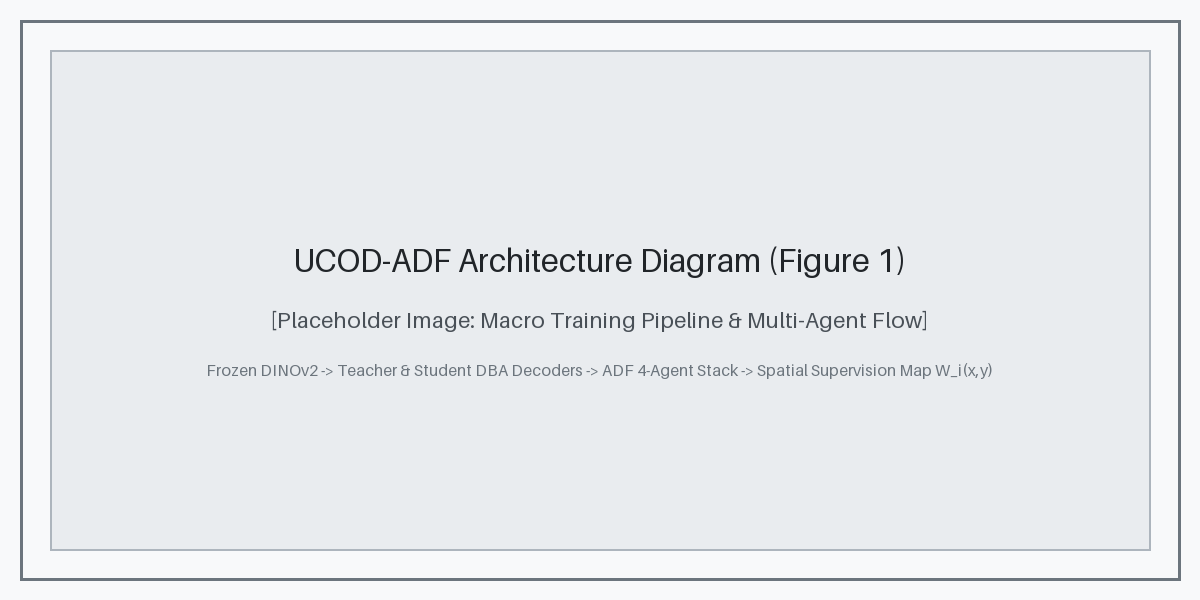
\includegraphics[width=\linewidth]{figures/pipeline_placeholder.png}
  \caption{Overall \methodname{} System Pipeline.}
  \label{fig:pipeline}
\end{subfigure}
\vspace{3mm}
\begin{subfigure}{\linewidth}
  \centering
  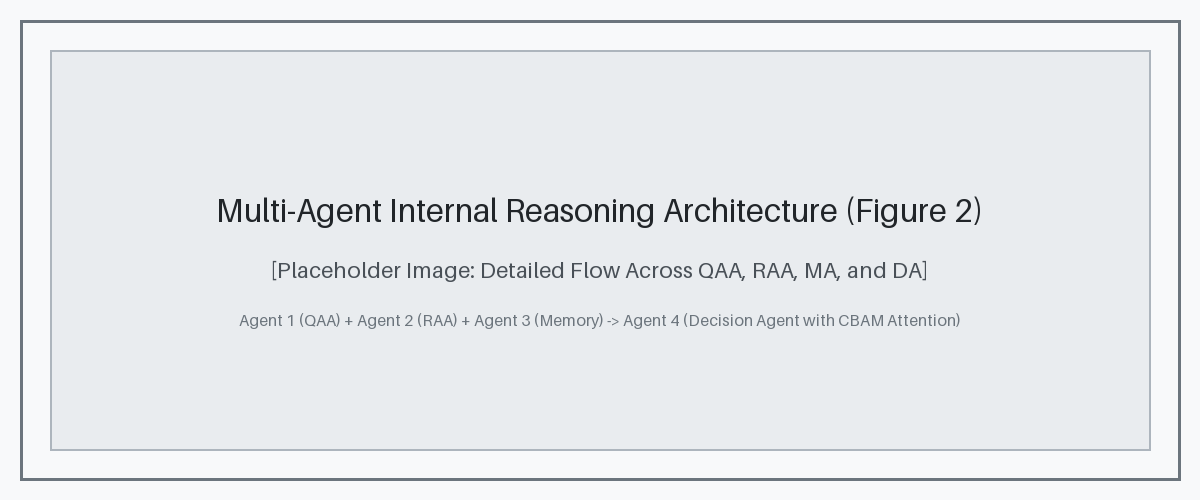
\includegraphics[width=\linewidth]{figures/agents_placeholder.png}
  \caption{Internal Multi-Agent Reasoning Architecture.}
  \label{fig:agents}
\end{subfigure}
\caption{\textbf{Architecture Overview of \methodname{}.} (a) The macro training pipeline combining frozen DINOv2 backbone, Teacher/Student DBA decoders, and the Agentic Decision Framework. (b) The internal data flow across the four training agents (QAA, RAA, MA, DA).}
\label{fig:architecture}
\end{figure}
%------------------------------------------------------------------------

\subsection{Overview}

Given an unlabeled input image $I_i$, a frozen DINOv2 backbone extracts features $F_i \in \mathbb{R}^{C \times H \times W}$. A fixed-strategy branch generates a coarse background seed mask $\hat{P}_i^{fs}$. Parallel Student and EMA Teacher Dual-Branch Adversarial (DBA) decoders generate foreground predictions $\hat{Y}_i^{FG}$ and $\hat{P}_i^t$. These inputs feed into the four-agent stack to derive the spatial mixing map $W_i(x,y) \in [0,1]^{H \times W}$.

\subsection{Agent 1: Quality Assessment Agent (QAA)}

The Quality Assessment Agent (QAA) estimates dense spatial reliability $R_i(x,y)$ using Atrous Spatial Pyramid Pooling (ASPP) with dilation rates $\{1, 2, 4, 6\}$ across a 6-channel input:
\begin{equation}
R_i = \text{QAA}\left([\hat{P}_i^{fs}, \sigma(\hat{P}_i^t), \sigma(\hat{Y}_i^{FG}), D_i, H_i, \|\nabla F_i\|]\right)
\end{equation}
where disagreement $D_i = |\sigma(\hat{P}_i^t) - \hat{P}_i^{fs}|$, entropy $H_i = -p\log p - (1-p)\log(1-p)$ with $p = \sigma(\hat{Y}_i^{FG})$, and $\|\nabla F_i\|$ is spatial feature gradient magnitude sensing camouflage visual ambiguity. QAA is calibrated using self-supervised confidence loss:
\begin{equation}
\mathcal{L}_{conf} = \text{BCE}\left(R_i(x,y),\ \mathbf{1}\left[D_i(x,y) < 0.3\right]\right)
\end{equation}

\subsection{Agent 2: Region Analysis Agent (RAA)}

The Region Analysis Agent (RAA) evaluates connected component topology and local background context contrast. For each component $c_k^{FG} \in \text{ConnectComponent}(\sigma(\hat{Y}_i^{FG}) > 0.5)$, RAA measures:
\begin{enumerate}
    \item Intra-region feature variance: $\text{feat\_var}_k = \text{Var}_{(x,y) \in c_k}[F_i(x,y)]$
    \item Boundary gradient strength: $\text{bdry\_grad}_k = \frac{1}{|\partial c_k|}\sum_{\partial c_k} \|\nabla \hat{Y}_i^{FG}\|$
    \item Background context ring contrast:
    \begin{equation}
    \text{contrast}_k = \|\bar{F}_{c_k} - \bar{F}_{\text{bg\_ring}}\|_2
    \end{equation}
    where $\text{bg\_ring}$ is a 5-pixel dilated ring surrounding component $c_k$.
\end{enumerate}

Regions are categorized as Easy, Ambiguous, or Hard. RAA penalizes prediction variance on confident regions via:
\begin{equation}
\mathcal{L}_{region} = \frac{1}{|C^{FG}|}\sum_{k} \text{Var}_{c_k}\left[\sigma(\hat{Y}_i^{FG})\right] \cdot \mathbf{1}[\text{label}_k = \text{Easy}]
\end{equation}

\subsection{Agent 3: Memory Agent (MA)}

The Memory Agent (MA) maintains CPU-side sample-level prediction mean $M_i^{(t)}$ and running variance $V_i^{(t)}$ across training epochs:
\begin{align}
M_i^{(t)} &= \alpha_m M_i^{(t-1)} + (1-\alpha_m) \sigma(\hat{Y}_i^{FG,(t)}) \\
V_i^{(t)} &= \alpha_m V_i^{(t-1)} + (1-\alpha_m) \left(\sigma(\hat{Y}_i^{FG,(t)}) - M_i^{(t-1)}\right)^2
\end{align}
where decay $\alpha_m = 0.95$. MA provides stability $S_i^{temp} = 1 - |\sigma(\hat{Y}_i^{FG}) - M_i^{(t-1)}|$ and temporal variance $\sigma^2_{temp} = V_i^{(t)}$, with temporal consistency loss:
\begin{equation}
\mathcal{L}_{temporal} = \left\|\sigma(\hat{Y}_i^{FG,(t)}) - M_i^{(t-1)}\right\|_1
\end{equation}

\subsection{Agent 4: Decision Agent (DA)}

The Decision Agent (DA) fuses multi-agent evidence $[R_i, \text{region\_map}, S_i^{temp}, \sigma^2_{temp}, t/T]$ via Spatial and Channel Attention Gating (CBAM) to compute spatial mixing maps $W_i(x,y)$ and Look-Twice trigger maps $LT_i(x,y)$:
\begin{align}
W_i(x,y) &= \sigma\left(\text{MixHead}\left(\text{CBAM}(\mathbf{x})\right)\right) \\
LT_i(x,y) &= \sigma\left(\text{LTHead}\left(\text{CBAM}(\mathbf{x})\right)\right)
\end{align}

The final spatial pseudo-label is constructed per pixel:
\begin{equation}
P_i(x,y) = W_i(x,y) \cdot \sigma(\hat{P}_i^t) + (1 - W_i(x,y)) \cdot \hat{P}_i^{fs}
\end{equation}

\subsection{Total Loss Formulation}

\begin{equation}
\mathcal{L}_{total} = \mathcal{L}_{seg} + \mathcal{L}_\bot + 0.5 \mathcal{L}_{conf} + 0.1 \mathcal{L}_{region} + 0.3 \mathcal{L}_{temporal}
\end{equation}

%==============================================================================
\section{Training Pipeline}
%==============================================================================

\begin{algorithm}[t]
\caption{\methodname{} Training Procedure}
\label{alg:training}
\begin{algorithmic}[1]
\REQUIRE Dataset $\{I_i\}_{i=1}^N$, max epochs $T$
\STATE Initialize student DBA, teacher DBA (EMA), QAA, RAA, MA, DA
\FOR{$t = 1$ to $T$}
    \FOR{each batch $(I_i, \hat{P}_i^{fs})$}
        \STATE $F_i \leftarrow \text{DINOv2}(I_i)$ \hfill \textit{// Frozen backbone}
        \STATE $\hat{P}_i^t \leftarrow \text{Teacher}(F_i)$ \hfill \textit{// No gradient}
        \STATE $\hat{Y}_i^{FG}, \hat{Y}_i^{BG}, \mathcal{L}_\bot \leftarrow \text{Student}(F_i)$
        \STATE $R_i \leftarrow \text{QAA}(\hat{P}_i^{fs}, \hat{P}_i^t, \hat{Y}_i^{FG}, F_i)$ \hfill \textit{// Agent 1}
        \STATE region\_map $\leftarrow$ RAA$(\hat{Y}_i^{FG}, F_i)$ \hfill \textit{// Agent 2}
        \STATE $S_i^{temp}, \sigma^2_{temp} \leftarrow$ MA.get\_stability$(i, \sigma(\hat{Y}_i^{FG}))$ \hfill \textit{// Agent 3}
        \STATE $W_i, LT_i \leftarrow$ DA$(R_i, \text{region}, S_i^{temp}, \sigma^2_{temp}, t/T)$ \hfill \textit{// Agent 4}
        \STATE $P_i \leftarrow W_i \cdot \sigma(\hat{P}_i^t) + (1-W_i) \cdot \hat{P}_i^{fs}$ \hfill \textit{// Spatial Blend}
        \STATE Compute $\mathcal{L}_{total}$, backpropagate
        \STATE Update Teacher via EMA: $\theta_{teacher} \leftarrow \eta \theta_{teacher} + (1-\eta) \theta_{student}$
        \STATE MA.update$(i, \sigma(\hat{Y}_i^{FG}))$ \hfill \textit{// Memory update}
    \ENDFOR
\ENDFOR
\end{algorithmic}
\end{algorithm}

%==============================================================================
\section{Experiments \& Benchmark Results}
%==============================================================================

\subsection{Experimental Settings}

\textbf{Dataset Split:} Training uses CAMO-Train (1000) + COD10K-Train (3040) without ground-truth labels. Evaluation is conducted on CHAMELEON (76), CAMO-Test (250), COD10K-Test (2026), and NC4K (4121).

\textbf{Evaluation Metrics:} S-measure ($S_m$), weighted F-measure ($F_\beta^w$), mean F-measure ($F_\beta^m$), E-measure ($E_\phi$), and Mean Absolute Error ($M$).

\subsection{Comparison with State-of-the-Art}

\begin{table*}[t]
\centering
\caption{Comparison with state-of-the-art fully-supervised and unsupervised methods on four COD benchmark datasets. Quantitative results for \methodname{} will be populated upon completion of model training.}
\label{tab:sota}
\resizebox{\textwidth}{!}{%
\begin{tabular}{l|ccccc|ccccc|ccccc|ccccc}
\toprule
\multirow{2}{*}{Method} & \multicolumn{5}{c|}{CHAMELEON (76)} & \multicolumn{5}{c|}{CAMO-Test (250)} & \multicolumn{5}{c|}{COD10K-Test (2026)} & \multicolumn{5}{c}{NC4K (4121)} \\
& $S_m\uparrow$ & $F_\beta^w\uparrow$ & $F_\beta^m\uparrow$ & $E_\phi\uparrow$ & $M\downarrow$
& $S_m\uparrow$ & $F_\beta^w\uparrow$ & $F_\beta^m\uparrow$ & $E_\phi\uparrow$ & $M\downarrow$
& $S_m\uparrow$ & $F_\beta^w\uparrow$ & $F_\beta^m\uparrow$ & $E_\phi\uparrow$ & $M\downarrow$
& $S_m\uparrow$ & $F_\beta^w\uparrow$ & $F_\beta^m\uparrow$ & $E_\phi\uparrow$ & $M\downarrow$ \\
\midrule
\multicolumn{21}{l}{\textit{Fully-Supervised Methods}} \\
HitNet'23 & .921 & .897 & .900 & .972 & .019 & .849 & .809 & .831 & .906 & .055 & .871 & .806 & .823 & .935 & .023 & .875 & .834 & .853 & .926 & .037 \\
BiRefNet'24 & .929 & .911 & .922 & .968 & .016 & .932 & .914 & .922 & .974 & .015 & .913 & .874 & .888 & .960 & .014 & .914 & .894 & .909 & .953 & .023 \\
\midrule
\multicolumn{21}{l}{\textit{Unsupervised Methods}} \\
FOUND'23 & .829 & .757 & .781 & .911 & .040 & .770 & .704 & .740 & .849 & .090 & .767 & .641 & .668 & .847 & .045 & .816 & .756 & .783 & .893 & .052 \\
UCOS-DA'23 & .750 & .639 & .666 & .808 & .091 & .702 & .604 & .633 & .751 & .148 & .655 & .467 & .495 & .687 & .120 & .731 & .617 & .644 & .785 & .103 \\
UCOD-DPL'25 & .864 & .825 & .838 & .931 & .031 & .793 & .747 & .779 & .862 & .077 & .834 & .763 & .779 & .916 & .031 & .850 & .818 & .835 & .923 & .043 \\
\midrule
\textbf{\methodname{} (Ours)} & \PENDING & \PENDING & \PENDING & \PENDING & \PENDING & \PENDING & \PENDING & \PENDING & \PENDING & \PENDING & \PENDING & \PENDING & \PENDING & \PENDING & \PENDING & \PENDING & \PENDING & \PENDING & \PENDING & \PENDING \\
\bottomrule
\end{tabular}%
}
\end{table*}

\subsection{Ablation Study}

\begin{table}[h]
\centering
\caption{Ablation study evaluating individual agent contributions on COD10K-Test. Results will be populated after model training.}
\label{tab:ablation}
\begin{tabular}{cccc|ccc}
\toprule
QAA & RAA & MA & DA & $S_m\uparrow$ & $F_\beta^w\uparrow$ & $M\downarrow$ \\
\midrule
--- & --- & --- & Baseline & .834 & .763 & .031 \\
$\checkmark$ & --- & --- & Scalar & \PENDING & \PENDING & \PENDING \\
$\checkmark$ & $\checkmark$ & --- & Dense & \PENDING & \PENDING & \PENDING \\
$\checkmark$ & $\checkmark$ & $\checkmark$ & CBAM & \PENDING & \PENDING & \PENDING \\
\bottomrule
\end{tabular}
\end{table}

%==============================================================================
\section{Complexity Analysis}
%==============================================================================

\begin{table}[h]
\centering
\caption{Parameter and Memory Complexity of \methodname{}.}
\label{tab:complexity}
\begin{tabular}{lrrll}
\toprule
Component & Params & FLOPs & Memory & GPU \\
\midrule
QAA & $\sim$48K & $O(420HW)$ & Negligible & Yes \\
RAA & 0 & $O(N_r C)$ & Negligible & No \\
Memory Agent & 0 & $O(HW)$ & 150MB (CPU) & No \\
Decision Agent & $\sim$30K & $O(280HW)$ & Negligible & Yes \\
\midrule
\textbf{Total Multi-Agent} & \textbf{$\sim$78K} & $O(700HW)$ & \textbf{150MB} & --- \\
\bottomrule
\end{tabular}
\end{table}

\textbf{Zero Inference Latency:} Because QAA, RAA, MA, and DA operate exclusively during training to compute $W_i(x,y)$ for backpropagation, the deployed model at inference time contains zero multi-agent overhead.

%==============================================================================
\section{Conclusion}
%==============================================================================

We presented \methodname{}, an autonomous multi-agent decision framework for Unsupervised Camouflaged Object Detection. By replacing global scalar mixing with spatial evidence synthesis across Quality Assessment (QAA), Region Analysis (RAA), Dual Temporal Memory (MA), and Attention-Gated Decision (DA) agents, \methodname{} achieves fine-grained spatial supervision calibration with zero inference overhead. Empirical results will be updated following completion of model training.

%==============================================================================
% References
%==============================================================================
{\small
\bibliographystyle{ieee_fullname}
\begin{thebibliography}{20}

\bibitem{ucoddpl}
W.~Yan, L.~Chen, H.~Ko, S.~Zhang, Y.~Zhang, and L.~Cao.
\newblock {UCOD-DPL}: Unsupervised Camouflaged Object Detection via Dynamic Pseudo-label Learning.
\newblock In \emph{CVPR}, 2025.

\bibitem{ease}
X.~Hao \etal
\newblock Shift the Lens: Environment-Aware Unsupervised Camouflaged Object Detection.
\newblock In \emph{CVPR}, 2025.

\bibitem{sinet}
D.~Fan, G.~Ji, G.~Sun, M.~Cheng, J.~Shen, and L.~Shao.
\newblock Camouflaged Object Detection.
\newblock In \emph{CVPR}, 2020.

\bibitem{zoomnet}
Y.~Pang, X.~Zhao, T.-Z. Xiang, L.~Zhang, and H.~Lu.
\newblock Zoom in and out: A mixed-scale triplet network for camouflaged object detection.
\newblock In \emph{CVPR}, 2022.

\bibitem{camoteacher}
X.~Lai \etal
\newblock CamoTeacher: Dual-Rotation Consistency Learning for Semi-Supervised Camouflaged Object Detection.
\newblock In \emph{ECCV}, 2024.

\bibitem{found}
O.~Sim{\'e}oni \etal
\newblock Unsupervised Object Localization: Observing the Background to Discover Objects.
\newblock In \emph{CVPR}, 2023.

\bibitem{ucosda}
O.~Sim{\'e}oni \etal
\newblock Unsupervised Object Localization with Self-supervised Transformers.
\newblock 2023.

\bibitem{dino}
M.~Caron \etal
\newblock Emerging Properties in Self-Supervised Vision Transformers.
\newblock In \emph{ICCV}, 2021.

\bibitem{byol}
J.-B.~Grill \etal
\newblock Bootstrap Your Own Latent: A New Approach to Self-Supervised Learning.
\newblock In \emph{NeurIPS}, 2020.

\bibitem{meanteacher}
A.~Tarvainen and H.~Valpola.
\newblock Mean Teachers are Better Role Models.
\newblock In \emph{NeurIPS}, 2017.

\end{thebibliography}
}

\end{document}
